\documentclass[pdf, aspectratio=169]{beamer}
\usepackage[]{hyperref,graphicx,siunitx,lmodern,booktabs,tikz,tensor}
\usepackage{pdfpc-commands}

\usepackage[mode=buildnew]{standalone}
\mode<presentation>{\usetheme{Astro}}

\graphicspath{ {../Images/} }

\sisetup{per-mode=symbol}
\usetikzlibrary{calc,intersections, decorations.pathmorphing,shadings,fadings}
\pgfdeclarehorizontalshading{rainbow}{100bp}{
  color(0bp)=(violet);
  color(30bp)=(black!30!violet); 
  color(38bp)=(blue);
  color(42bp)=(black!20!cyan);
  color(46bp)=(green); 
  color(52bp)=(yellow);
  color(58bp)=(orange);
  color(65bp)=(red); 
  color(73bp)=(black!60!red);
  color(100bp)=(black!50!red)
}

\newcommand{\linespectra}[2]{
  \coordinate (init) at (#1);
  \fill[shading=rainbow, opacity=0.1] (init) rectangle +(4,1);
  \draw[black,very thick] (init) rectangle +(4,1);
  \foreach \f in {#2}{
	\definecolor{col}{wave}{\f}
	%\fill[left color=transparent,right color=transparent,middle color=col] ($(init)+(\f/100-4,0)$) rectangle +(0.5mm,1cm);
	\fill[col, path fading=east] ($(init)+(\f/100-4+0.025,0)$) rectangle +(0.25mm,1cm);
	\fill[col, path fading=west] ($(init)+(\f/100-4+0.025,0)$) rectangle +(-0.25mm,1cm);
	%\node[white,anchor=west,font=\tiny, rotate=-90] at ($(init)+(\f/100-4+0.025,0)$) {\f nm};
  }
}

\newcommand{\absorbspectra}[2]{
  \coordinate (init) at (#1);
  \fill[shading=rainbow, opacity=0.8] (init) rectangle +(4,1);
  \draw[black,very thick] (init) rectangle +(4,1);
  \foreach \f in {#2}{
	\definecolor{col}{wave}{900}
	%\fill[left color=transparent,right color=transparent,middle color=col] ($(init)+(\f/100-4,0)$) rectangle +(0.5mm,1cm);
	\fill[col, path fading=east] ($(init)+(\f/100-4+0.025,0)$) rectangle +(0.25mm,1cm);
	\fill[col, path fading=west] ($(init)+(\f/100-4+0.025,0)$) rectangle +(-0.25mm,1cm);
	%\node[white,anchor=west,font=\tiny, rotate=-90] at ($(init)+(\f/100-4+0.025,0)$) {\f nm};
  }
}
%\tikzstyle{proton}=[circle, minimum size = 7mm, ball color=red, black,transform shape]
%\tikzstyle{neutron}=[circle, minimum size=7mm, ball color=gray, black, transform shape]
%\tikzstyle{gammaray}=[ultra thick, -latex, decorate, decoration={snake, post length=3mm}]


%preamble
\title{Through the Looking Glass}
\date{September 24, 2018}
\author{Jed Rembold}

\begin{document}
\renewcommand*{\theenumi}{\Alph{enumi}}

\begin{frame}{Announcements}
  \begin{itemize}
	  \item WebWorK due Wednesday
	  \item Test on Friday!
		  \begin{itemize}
		  	\item Study materials have been posted
			\item Solutions to study materials have been posted
			\item Equation sheet is posted
			\item You need to bring writing implements, a basic calculator (can't be your phone) and a positive attitude!
				\begin{itemize}
					\item Email me if you'd like to use one of my limited number of backup calculators
				\end{itemize}
			\item Today is the last day of content which is testable
		  \end{itemize}
	  \item Lab tonight is on Light, which \alert{is} on the test
	\item Polling: \url{rembold-class.ddns.net}
  \end{itemize}
\end{frame}

\begin{frame}{Astronomy News!}
	\begin{columns}
		\column{0.5\textwidth}
		\begin{itemize}
			\item JAXA deploys two small rovers to the surface of asteroid Ryugu!
			\item Orbiter lowered to about 55 meters to drop off rovers and then resumed orbit
			\item Rovers move by ``hopping'' in the weak gravity
			\item Third larger rover to be released in October
		\end{itemize}
		
		\column{0.5\textwidth}
		\begin{center}
			\includegraphics[width=\textwidth]{JAXA_Rover.jpg}
		\end{center}
		
	\end{columns}
\end{frame}

\begin{frame}{Review Question}
	The image below is a normal spectrum, and then the second is the observed spectrum of a distant star. How is the star moving relative to Earth?
	\begin{center}
		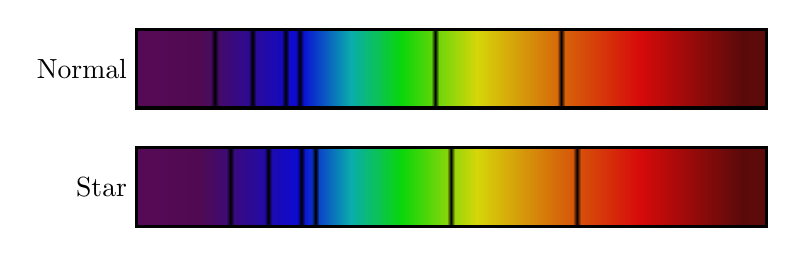
\begin{tikzpicture}[xscale=2]
		  \absorbspectra{0,0}{447,471,492,501,587,667}
		  \node[anchor=east] at (0,.5) {Normal};
		  \absorbspectra{0,-1.5}{457,481,502,511,597,677}
		  \node[anchor=east] at (0,-1) {Star};
		\end{tikzpicture}
	\end{center}
	\begin{enumerate}
		\item \alert<2>{Away from us}
		\item Towards us
		\item Not moving at all
		\item Only moving sideways to us
	\end{enumerate}
\end{frame}

\begin{frame}{Telescopes for Visual Observing}
  \begin{itemize}
	\item If using your eye as your ``detector'' on a telescope, then the optics is a bit more complicated
	\item Need an eye-piece to make the light rays parallel again so that your eyeball can then process them correctly
  \end{itemize}
  \begin{center}
	\includegraphics[width=.6\textwidth]{ch16_telescope_optics.pdf}
  \end{center}
\end{frame}

\begin{frame}{Refracting Telescopes}
  \begin{columns}
	\column{.5\textwidth}
	\begin{itemize}
	  \item Use a lens to focus light
	  \item Classic and simple style
	  \item Difficult to make very large
		\begin{itemize}
		  \item Lenses get huge and heavy
		\end{itemize}
	\end{itemize}
	\begin{center}
	  \includegraphics[width=.8\textwidth]{ch16_refractor_im.jpg}
	\end{center}
	\column{.5\textwidth}
	\begin{center}
	  \begin{tikzpicture}[scale=.9, transform shape]
		\node[rotate=-30] at (0,0) {\includegraphics[width=1.5cm]{ch16_refractor.pdf}};
		\draw[orange] (-1.5,-3) --+(10:1) node[right] {Eye-piece};
		\node[yellow,align=center,rotate=-30, font=\scriptsize] at (2,3.5) {To the\\Stars!};
	  \end{tikzpicture}
	\end{center}
  \end{columns}
\end{frame}

\begin{frame}{Reflecting Telescopes}
  \begin{columns}
	\column{.5\textwidth}
	\begin{center}
	  \begin{tikzpicture}[scale=.9, transform shape]
		\node[rotate=-30] at (0,0) {\includegraphics[width=2cm]{ch16_reflector.pdf}};
		\draw[orange] (0,2) --+(135:1) node[left] {Eye-piece};
		\draw[orange] (-.5,-3) --+(10:1) node[right] {Primary Mirror};
		\draw[orange] (1.25,1.25) --+(280:2) node[below,align=center] {Secondary\\Mirror};
		\node[yellow,align=center,rotate=-30, font=\scriptsize] at (2.15,3) {To the\\Stars!};
	  \end{tikzpicture}
	\end{center}
	\column{.5\textwidth}
	\begin{itemize}
	  \item Use a mirror as the primary means of focusing light
	  \item Can be made quite large!
	  \item Variant with hole in primary mirror
		\begin{itemize}
		  \item Schmidt-Cassegrain
		\end{itemize}
	\end{itemize}
	\begin{center}
	  \includegraphics[width=.7\textwidth]{ch16_reflector_im.jpg}
	\end{center}
  \end{columns}
\end{frame}

\begin{frame}{Optical Telescope Example: MRO}
  \begin{center}
	\includegraphics<1>[width=.65\textwidth]{ch16_MRO3.jpg}
	\includegraphics<2>[width=.5\textwidth]{ch16_MRO2.jpg}
	\includegraphics<3>[width=.9\textwidth]{ch16_MRO1.jpg}
  \end{center}
\end{frame}

\begin{frame}{Radio Telescope Example: VLA}
  \begin{center}
	\includegraphics<1>[width=.4\textwidth]{ch16_VLA1.jpg}
	\includegraphics<2>[width=\textwidth]{ch16_VLA2.jpg}
  \end{center}
\end{frame}

\begin{frame}{Imaging: What You Care About}
  \begin{columns}
	\column{.6\textwidth}
	\begin{itemize}
	  \item \alert{Aperture Size:} the light collecting area
	  \item \alert{Angular Resolution:} how much angular detail you can see
	  \item \alert{Field of View:} how much of the sky you can see at once
	\end{itemize}
	\column{.4\textwidth}
	\begin{center}
	  \includegraphics[width=.8\textwidth]{ch16_angular_resolution.png}
	\end{center}
  \end{columns}
\end{frame}

\begin{frame}{Aperture Size}
  \begin{itemize}
	\item Related to the size of the telescope
	\item Or more precisely, to the size of the telescope's primary mirror
	\item A larger telescope will gather more light in a particular amount of time, bringing out dim details or brightening the image in general
  \end{itemize}
  \begin{center}
	\includegraphics[width=.5\textwidth]{ch16_aperturesize.jpg}
  \end{center}
\end{frame}

\begin{frame}{Angular Resolution: The Diffraction Limit}
  \begin{itemize}
	\item Light behaves in part like a wave
	  \begin{itemize}
		\item Light passing through any opening thus has its rays bent slightly
	  \end{itemize}
	  \begin{center}
		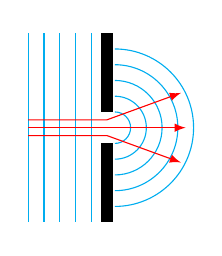
\begin{tikzpicture}
		  \draw[line width=4pt] (0,2mm) --+(0,1) (0,-2mm) --+(0,-1);
		  \foreach \x in {-.2, -.4, ..., -1}{
			\draw[cyan] (\x,1.2) --+(0,-2.4);
		  }
		  \foreach \r in {.2,.4,...,1}{
			\draw[cyan] (.1,\r) arc(90:-90:\r);
		  }
		  \onslide<2>{
			\draw[red, -latex] (-1,1mm) -- (0,1mm) --+(20:1);
			\draw[red, -latex] (-1,0) -- +(2,0);
			\draw[red, -latex] (-1,-1mm) -- (0,-1mm) --+(-20:1);
		  }
		\end{tikzpicture}
	  \end{center}
	\item The \underline{Diffraction Limit} depends on the ratio of the wavelength to opening
	  \[\text{Smallest Angle} \propto \frac{\text{Wavelength}}{\text{Diameter of Opening}}\]
  \end{itemize}
\end{frame}

\begin{frame}{Size Does Matter}
  \begin{itemize}
	\item Larger telescopes have a smaller diffraction limit and thus greater angular resolution
	\item But ground based optical telescopes are more limited by atmospheric effects
	\item Radio telescopes need to be large for good angular resolution owing to the large wavelength of radio waves
  \end{itemize}
  \begin{columns}
	\column{.5\textwidth}
	\begin{center}
	  \includegraphics[width=.75\textwidth]{ch16_Arecibo.jpg}
	\end{center}
	\column{.5\textwidth}
	\begin{center}
	  \includegraphics[width=.8\textwidth]{ch16_VLA3.jpg}
	\end{center}
  \end{columns}
\end{frame}

\begin{frame}{Magnification vs Field of View}
  \begin{itemize}
	\item Magnification and Field of View are inversely related
	  \begin{itemize}
		\item One goes up, the other goes down
	  \end{itemize}
	\item Eye-piece optics primarily responsible for magnification
	  \begin{itemize}
		\item Increases the apparent size of the object
		\item Can help overcome diffraction limits of your eye
	  \end{itemize}
  \end{itemize}
  \begin{center}
	\begin{tikzpicture}[scale=.9, transform shape]
	  \node[inner sep=0pt, outer sep=0pt,anchor=south] (r) at (-1,0) {\includegraphics[width=1cm]{ch16_rocket.png}};
	  \fill[cyan!50] (0,-2) arc(-15:15:8) arc (165:195:8);
	  \node[red] (f1) at (-2,0) {$\otimes$};
	  \node[red] (f2) at (2,0) {$\otimes$};
	  \draw[yellow] (r.north) -- ($(r.north)!-1.45cm!(f1)$) coordinate (mid2) --+(3,0);
	  \draw[yellow] (r.north) --+(1,0) coordinate (mid) -- ($(mid)!1.3!(f2)$);
	  \draw<2->[yellow, dashed] (mid2) --+(-3,0);
	  \draw<2->[yellow, dashed] (f2) -- ($(f2)!2.5!(mid)$);
	  \node<3->[inner sep=0pt, outer sep=0pt, anchor=south, opacity=0.7] at (-2,0) {\includegraphics[width=2cm]{ch16_rocket.png}};
	  \node[inner sep=0pt, outer sep=0pt] at (3.3,1) {\includegraphics[width=3cm]{ch16_eye-side.png}};
	\end{tikzpicture}
  \end{center}
\end{frame}

\begin{frame}{What Do We Mean By ``Seeing''}
  \begin{itemize}
	\item Atmospheric variations limit angular resolution of optical telescopes on Earth
	  \begin{itemize}
		\item Makes stars twinkle
		\item Distorts the rays cast from the star
	  \end{itemize}
	\item ``Seeing'' describes how calm the nightly atmospheric distortion is
	  \begin{itemize}
		\item Excellent Seeing has minimal distortion (Left)
		\item Poor Seeing has very obvious distortion (Right)
	  \end{itemize}
  \end{itemize}
  \begin{columns}
	\column{.5\textwidth}
	\begin{center}
	  \inlineMovie{../Videos/Seeing_Ex.ogv}{../Videos/Seeing_Ex.png}{width=.75\textwidth}
	\end{center}
	\column{.5\textwidth}
	\begin{center}
	  \inlineMovie{../Videos/Seeing_Poor.ogv}{../Videos/Seeing_Poor.png}{width=.75\textwidth}
	\end{center}
  \end{columns}
\end{frame}

\begin{frame}{Where the View is Better}
  \begin{columns}
	\column{.5\textwidth}
	\begin{itemize}
	  \item Best seeing on Earth is a fraction of an arcsecond
	  \item Even small telescopes in space are useful!
	\end{itemize}
	\column{.5\textwidth}
	\begin{center}
	  \begin{tikzpicture}
		\node[inner sep=0pt, outer sep=0pt] at (0,0) {\includegraphics[width=7cm]{ch16_Seeing.png}};
		\node[cyan, anchor=south, font=\scriptsize] at (-1.75,3) {Subaru (8m)};
		\node[orange, anchor=south, font=\scriptsize] at (1.75,3) {Hubble (2.4m)};
	  \end{tikzpicture}
	\end{center}
  \end{columns}
\end{frame}

\begin{frame}{Interferometry}
	\begin{itemize}
		\item Requires many telescopes working together
		\item Light waves interfere with one another when they enter the telescope
		\item Can electronically reconstruct the data from many telescopes
		\item Radio:
			\begin{itemize}
				\item VLA
				\item VLBA
			\end{itemize}
		\item Millimeter:
			\begin{itemize}
				\item ALMA
			\end{itemize}
	\end{itemize}
\end{frame}

\begin{frame}{VLA Resolutions}
	\begin{center}
		\includegraphics[width=0.8\textwidth]{Ch6_VLA_Example.png}
	\end{center}
\end{frame}

\begin{frame}{VLBA}
	\begin{center}
		\includegraphics[width=0.65\textwidth]{Ch6_VLBA.png}
	\end{center}
\end{frame}

\begin{frame}{ALMA}
	\begin{center}
		\includegraphics[width=0.7\textwidth]{Ch6_Alma.jpeg}
	\end{center}
\end{frame}

\begin{frame}{Test Questions?}
	Anything you want to ask or review?
\end{frame}

%\begin{frame}{To Add Still}
	%\begin{itemize}
		%\item Spectroscopy
		%\item Interferometry
		%\item Future Large Telescopes!
	%\end{itemize}
%\end{frame}
	



\end{document}
